\documentclass[a4paper,11pt]{article}
\usepackage[spanish]{babel}
\usepackage[utf8]{inputenc}

% Configuración páginas
\usepackage{vmargin}				% Márgenes

\usepackage{sectsty}				% Fuente de los títulos
\allsectionsfont{\normalfont \Large \scshape}

\usepackage{graphicx}				% Imágenes
\graphicspath{{images/}}

\usepackage{mathtools}				% Matematicas
\newcommand\numberthis{				% numeración en align*
	\addtocounter{equation}{1}\tag{\theequation}
}

% Configuración del título
\newcommand{\horrule}[1]{\rule{\linewidth}{#1}} 	% Horizontal rule

\title{
	\vspace{-25pt}
	\normalfont \Large \textsc{
		Modelos de Investigación Operativa,
        Ingeniería Informática\\
        Universidad de Valladolid
	}\\[10pt]
	\horrule{1pt}\\[10pt]
	\huge \textbf{
		Práctica 1
	}\\
	\horrule{1pt}
}
\author{
	\normalfont \Large Daniel González Alonso
}
\date{
	\normalfont \large \today
}

%%%%%%%%%%%%%%%%%%%%%%%%%%%%%%%%%%%%%%%%%%%%%%%%%%
\begin{document}
\maketitle

%%%% RESUMEN %%%%
\begin{abstract}
En este documento se describen los problemas y los resultados obtenidos de la práctica 1 del tema 2 de la asignatura Modelos de Investigación Operativa de Ingeniería Informática, Universidad de Valladolid.
\end{abstract}

%%%% DESARROLLO %%%%
\section{Introducción}

Esta práctica consiste en aplicar el modelo empleado en Set Covering a problemas con distancias. El modelo empleado para los problemas de Set Covering es el siguiente:

\begin{align*}\numberthis
   	&\textrm{Minimizar }	&& \sum_{j=1}^{n}{f_j \cdot x_j} \\
   	&\textrm{Sujeto a }		&& \sum_{j \in N_{i}}{a_{i,j} \cdot x_{j} \geq 1} 	&& i=1,\ldots,m \\
	&						&& x_{j} \in \{0,1\}					&& j=1,\ldots,n
\end{align*}

Donde ${m}$ es el número de puntos de demanda, ${n}$ es el número de posibles puntos de servicio, ${f_j}$ representa el coste de instalar un punto de servicio en ${j}$ y la matriz ${a_{i,j}}$ contiene solo los valores 1 si ${i}$ está cubierto por ${j}$ o 0 en caso contrario.\\

\section{Ejercicios}

El problema que tenemos que resolver para este apartado mediante el modelo anterior empleará los datos del archivo \texttt{matriz30x30.dat} donde se encuentran las distancias entre 30 unidades de población (condados) del estado de New York. La práctica consta de dos partes:

\newpage
\subsection{Parte 1}
Para una distancia de cubrimiento fija, hay que resolver el problema de cubrimiento total, buscando el mínimo número de instalaciones o puntos de servicio, de forma que todo condado quede cubierto a una distancia de 50 Km como máximo.

\begin{itemize}\item[]
En este problema, al tratarse de un problema de minimización de número de instalaciones y no de costes, ${f_j}$ siempre vale 1, y ${a_{i,j}}$ vale 1 si la distancia entre ${i}$ y ${j}$ es menor que la distancia ${dc=50}$.\\

El problema se resolvió mediante \textit{Xpress Mosel} en el archivo \texttt{NewYork\_part1.mos}. Los resultados obtenidos fueron que el número mínimo de instalaciones de puntos de servicio es de 18, situados en los condados 2, 4, 5, 9, 10, 11, 12, 13, 14, 16, 17, 18, 21, 22, 27, 28, 29 y 30.
\end{itemize}

\subsection{Parte 2}
Resolver el problema para todos los posibles valores de ${dc}$ desde 1 hasta 250, y construir la gráfica o tabla del número de instalaciones en función de la distancia de cubrimiento.

\begin{itemize}\item[]
El problema fue resuelto mediante \textit{Xpress Mosel} en el archivo \texttt{NewYork\_part2.mos}, donde se resuelve el mismo problema que en el apartado anterior pero iterando la distancia ${dc}$ entre los valores 1 y 250. Las respuestas obtenidas se almacenan en un archivo CSV en el cual podemos encontrar como columnas las distancias y su respectivo número de instalaciones. Con estos datos se creó la siguiente gráfica:

\begin{figure}[!htbp]
	\centering
	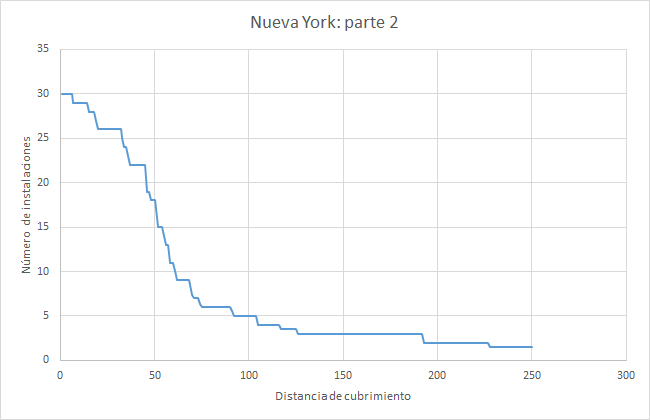
\includegraphics[width=1\textwidth]{NewYork_part2.png}
\end{figure}

Como se puede observar, cuanto mayor es la distancia de cubrimiento, menor es el número de instalaciones necesarias.
\end{itemize}

\end{document}
